\documentclass[../DoAn.tex]{subfiles}
\begin{document}

\section{Đặt vấn đề}
\label{section:1.1}

Ngày nay, sự phát triển của khoa học công nghệ ngày càng trở nên mạnh mẽ, đặc biệt với sự xuất hiện của Cách mạng Công nghiệp 4.0. Một trong số các công nghệ nổi bật nhất trong cuộc Cách mạng Công nghiệp lần thứ 4 này là IoT (Internet of Things). Năm 1999, Kevin Ashton \cite{KevinAshton} đã đưa ra cụm từ “Internet of Things” để mô tả hệ thống mà Internet được kết nối với thế giới vật chất thông qua các cảm biến. Từ năm 1999 đến nay, các thiết bị IoT được lắp đặt và sử dụng rất nhiều và đã tăng mạnh qua từng năm. Khi đó, với số lượng thiết bị tăng lên, độ trễ khi truyền tín hiệu từ bộ điều khiển tới các thiết bị sẽ càng nhiều lên dẫn tới chất lượng hoạt động của các thiết bị bị ảnh hưởng nhiều, năng suất hoạt động giảm sút và có thể dẫn tới xung đột. Bên cạnh đó, bộ điều khiển các thiết bị cũng là một vấn đề cần được nghiên cứu và phát triển để phía người dùng dễ dàng tiếp cận, sử dụng và phản hồi một cách tốt nhất. 

\begin{figure}[H]
    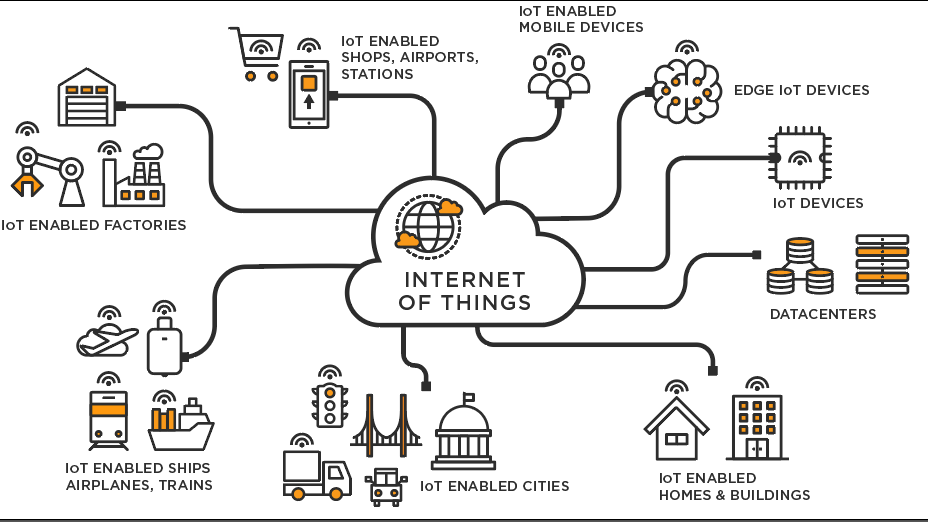
\includegraphics[width=0.9\linewidth]{Hinhve/IoT.png}
    \centering
    \caption{Biểu đồ use case tổng quát}
\end{figure}

Tại thời điểm hiện tại, nhiều công ty, tổ chức đã xây dựng, phát triển được các ứng dụng mobile phù hợp với những người dùng thường xuyên sử dụng điện thoại thông minh để các công việc điều khiển được tiện lợi hơn.
Tuy nhiên, việc phát triển ứng dụng có chi phí không hề rẻ, đặc biệt nếu công ty muốn xây dựng ở nhiều nền tảng như Android, iOS, Website sẽ phải tốn rất nhiều nhân công, chi phí, thời gian và nâng cấp. Vì vậy, trong đồ án này, em đã đề xuất xây dựng hệ thống điều khiển thiết bị Arduino bằng ứng dụng đa nền tảng - Android, iOS, Web thông qua một server có sử dụng socket để có thể xây dựng 1 ứng dụng chạy được nhiều nền tảng nhưng chỉ cần quản lý một mã nguồn, đồng thời sử dụng socket để cải thiện tính real-time giữa các thiết bị.

\section{Mục tiêu và phạm vi đề tài}
\label{section:1.2}
Với những vấn đề đã trình bày trong mục 1.1, trong ĐATN này em sẽ phát triển hệ thống ứng dụng điều khiển xe Arduino, ứng dụng có chức năng điều khiển xe Arduino. Các nhóm chức năng chính dự định sẽ triển khai là:
\begin{itemize}
\item Thứ nhất, ứng dụng sẽ kết nối với server, người dùng cần chọn một trong hai loại server là localhost hoặc web đã được công khai.
\item Thứ hai, người dùng có thể điều khiển thiết bị bằng giao diện trực quan trên ứng dụng, có thể điều khiển bằng giọng nói với câu lệnh đơn giản.
\item Thứ ba, người dùng có thể cài đặt tốc độ của xe, điều khiển đèn LED.
\item Thứ tư, server được xây dựng có sử dụng Socket.IO\cite{SocketIO} giúp nhận tín hiệu real-time từ ứng dụng.
\item Thứ năm, thiết bị Arduino hai bánh, một bánh điều hướng có kết nối wifi và server nhận tín hiệu real-time.
\end{itemize}

Để phát triển được một ứng dụng có thể đáp ứng được các chức năng trên, ứng dụng cần thiết kế và triển khai kiến trúc đáp ứng được tính liên tục, tức thì và ổn định, bên cạnh đó là dễ dàng mở rộng. Đồng thời, giao diện của ứng dụng được thiết kế đẹp mắt, tối giản mà dễ sử dụng để không gây ra nhiều khó khăn với người dùng, đặc biệt là những người mới tiếp xúc với công nghệ, từ đó tăng trải nghiệm người dùng. Và điểm không thể thiếu của ứng dụng là yêu cầu về kĩ thuật, bảo trì, sửa lỗi và nâng cấp tính năng về sau để không ảnh hưởng quá nhiều tới quá trình hoạt động của ứng dụng. 


\section{Định hướng giải pháp}
\label{section:1.3}
Với việc xây dựng hệ thống ứng dụng điều khiển thiết bị Arduino theo mục tiêu đã trình bày ở phần trên, em đã định hướng xây dựng nền tảng ứng dụng mobile cho người dùng và thiết bị Arduino thực hiện chức năng của nó.
Mã nguồn của hệ thống sẽ được chia làm 3 phần:
\begin{itemize}
\item Giao diện mobile: Hiển thị giao diện, người dùng tương tác và cập nhật dữ liệu.
\item Backend: nhận tín hiệu từ mobile truyền đến, xử lý và truyền tới thiết bị Arduino.
\item Thiết bị Arduino: Kết nối Wifi, nhận tín hiệu từ server và thực hiện các chức năng theo yêu cầu.
\end{itemize}

Phần ứng dụng Mobile sử dụng Flutter\cite{Flutter} – mobile UI framework của Google với ngôn ngữ lập trình Dart\cite{Dart}. Flutter cho phép ứng dụng hoạt động trên cả các nền tảng Android, iOS và Web.

Phần backend được xây dựng trên nền tảng NodeJs\cite{NodeJS}, sử dụng ngôn ngữ lập trình JavaScript. JavaScript với các ưu điểm như: ngôn ngữ lập trình nhẹ, phản hồi ngay lập tức, ... sẽ giúp hệ thống kết nối giữa ứng dụng và thiết bị có hiệu năng tốt tới người sử dụng. Ngoài ra, hệ thống có sử dụng Socket.IO để nhận tín hiệu từ ứng dụng một cách tức thì và ổn định.

Thiết bị Arduino đương xây dựng dựa trên Module NodeMCU Esp32\cite{ESP32-WROOM-32}, linh kiện này hỗ trợ kết nối với Wifi để có thể nhận tín hiệu từ Internet. Mã nguồn cho Arduino sử dụng Socket.IO để nhận tín hiệu tức thì từ server trả về.

\section{Bố cục đồ án}
\label{section:1.4}
Phần còn lại của Báo cáo Đồ án tốt nghiệp này được tổ chức như sau. 

Chương 2 trình bày về tổng quan các chức năng trong hệ thống đồng thời đặc tả một số use case chính.

Chương 3, em sẽ trình bày các công nghệ đã được sử dụng trong quá trình xây dựng và hoàn thành đồ án. Với mỗi công nghệ sẽ có cơ sở lý thuyết, công dụng cũng như lý do để sử dụng trong ĐATN này.

Chương 4 sẽ tập trung trình bày chi tiết về phân tích thiết kế hệ thống và trình bày sâu hơn về luồng hoạt động của một số nghiệp vụ chính trong hệ thống, thiết kế giao diện, thiết kế lớp, sau đó là triển khai và cuối cùng là kiểm thử.

Chương 5 trình bày về các giải pháp và đóng góp nổi bật của cá nhân với ĐATN này, đồng thời nêu ra các khó khăn và cách giải quyết những khó khăn đó trong quá trình hoàn thành ĐATN.

Cuối cùng, chương 6 là phần kết luận, chương này sẽ tổng kết lại quá trình xây dựng ứng dụng, những ưu, nhược điểm đã đạt được cũng như định hướng phát triển mở rộng trong tương lai.

\end{document}